% Created by tikzDevice version 0.10.1 on 2017-12-07 13:27:59
% !TEX encoding = UTF-8 Unicode
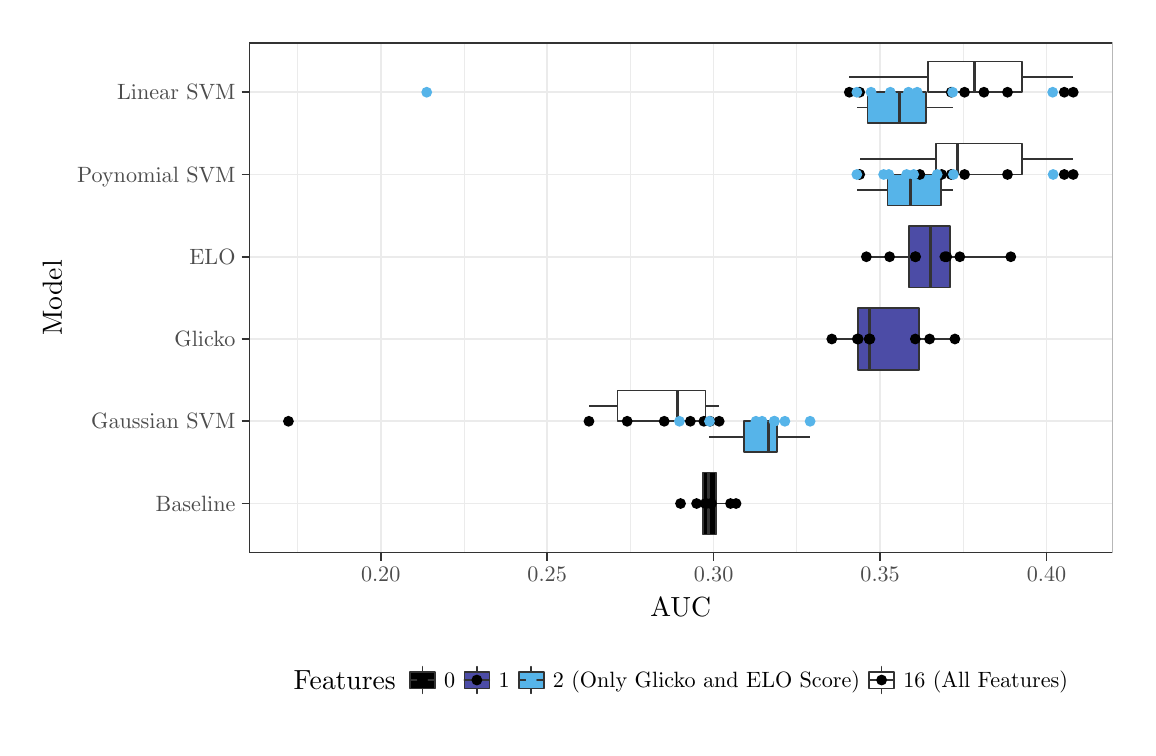
\begin{tikzpicture}[x=1pt,y=1pt]
\definecolor{fillColor}{RGB}{255,255,255}
\path[use as bounding box,fill=fillColor,fill opacity=0.00] (0,0) rectangle (397.48,252.94);
\begin{scope}
\path[clip] (  0.00,  0.00) rectangle (397.48,252.94);
\definecolor{drawColor}{RGB}{255,255,255}
\definecolor{fillColor}{RGB}{255,255,255}

\path[draw=drawColor,line width= 0.6pt,line join=round,line cap=round,fill=fillColor] (  0.00, -0.00) rectangle (397.48,252.94);
\end{scope}
\begin{scope}
\path[clip] ( 80.05, 63.15) rectangle (391.98,247.44);
\definecolor{fillColor}{RGB}{255,255,255}

\path[fill=fillColor] ( 80.05, 63.15) rectangle (391.98,247.45);
\definecolor{drawColor}{gray}{0.92}

\path[draw=drawColor,line width= 0.3pt,line join=round] ( 97.48, 63.15) --
	( 97.48,247.44);

\path[draw=drawColor,line width= 0.3pt,line join=round] (157.64, 63.15) --
	(157.64,247.44);

\path[draw=drawColor,line width= 0.3pt,line join=round] (217.80, 63.15) --
	(217.80,247.44);

\path[draw=drawColor,line width= 0.3pt,line join=round] (277.95, 63.15) --
	(277.95,247.44);

\path[draw=drawColor,line width= 0.3pt,line join=round] (338.11, 63.15) --
	(338.11,247.44);

\path[draw=drawColor,line width= 0.6pt,line join=round] ( 80.05, 80.99) --
	(391.98, 80.99);

\path[draw=drawColor,line width= 0.6pt,line join=round] ( 80.05,110.71) --
	(391.98,110.71);

\path[draw=drawColor,line width= 0.6pt,line join=round] ( 80.05,140.44) --
	(391.98,140.44);

\path[draw=drawColor,line width= 0.6pt,line join=round] ( 80.05,170.16) --
	(391.98,170.16);

\path[draw=drawColor,line width= 0.6pt,line join=round] ( 80.05,199.89) --
	(391.98,199.89);

\path[draw=drawColor,line width= 0.6pt,line join=round] ( 80.05,229.61) --
	(391.98,229.61);

\path[draw=drawColor,line width= 0.6pt,line join=round] (127.56, 63.15) --
	(127.56,247.44);

\path[draw=drawColor,line width= 0.6pt,line join=round] (187.72, 63.15) --
	(187.72,247.44);

\path[draw=drawColor,line width= 0.6pt,line join=round] (247.88, 63.15) --
	(247.88,247.44);

\path[draw=drawColor,line width= 0.6pt,line join=round] (308.03, 63.15) --
	(308.03,247.44);

\path[draw=drawColor,line width= 0.6pt,line join=round] (368.19, 63.15) --
	(368.19,247.44);
\definecolor{drawColor}{gray}{0.20}

\path[draw=drawColor,line width= 0.6pt,line join=round] (248.80, 80.99) -- (253.97, 80.99);

\path[draw=drawColor,line width= 0.6pt,line join=round] (244.08, 80.99) -- (241.71, 80.99);
\definecolor{fillColor}{RGB}{0,0,0}

\path[draw=drawColor,line width= 0.6pt,line join=round,line cap=round,fill=fillColor] (248.80, 69.84) --
	(244.08, 69.84) --
	(244.08, 92.14) --
	(248.80, 92.14) --
	(248.80, 69.84) --
	cycle;

\path[draw=drawColor,line width= 1.1pt,line join=round] (246.01, 69.84) -- (246.01, 92.14);

\path[draw=drawColor,line width= 0.6pt,line join=round] (270.81,105.14) -- (282.73,105.14);

\path[draw=drawColor,line width= 0.6pt,line join=round] (258.96,105.14) -- (246.36,105.14);
\definecolor{fillColor}{RGB}{86,180,233}

\path[draw=drawColor,line width= 0.6pt,line join=round,line cap=round,fill=fillColor] (270.81, 99.57) --
	(258.96, 99.57) --
	(258.96,110.71) --
	(270.81,110.71) --
	(270.81, 99.57) --
	cycle;

\path[draw=drawColor,line width= 1.1pt,line join=round] (267.56, 99.57) -- (267.56,110.71);

\path[draw=drawColor,line width= 0.6pt,line join=round] (244.90,116.29) -- (249.88,116.29);

\path[draw=drawColor,line width= 0.6pt,line join=round] (213.18,116.29) -- (202.82,116.29);
\definecolor{fillColor}{RGB}{255,255,255}

\path[draw=drawColor,line width= 0.6pt,line join=round,line cap=round,fill=fillColor] (244.90,110.71) --
	(213.18,110.71) --
	(213.18,121.86) --
	(244.90,121.86) --
	(244.90,110.71) --
	cycle;

\path[draw=drawColor,line width= 1.1pt,line join=round] (234.73,110.71) -- (234.73,121.86);

\path[draw=drawColor,line width= 0.6pt,line join=round] (322.04,140.44) -- (335.05,140.44);

\path[draw=drawColor,line width= 0.6pt,line join=round] (300.03,140.44) -- (290.57,140.44);
\definecolor{fillColor}{RGB}{76,76,166}

\path[draw=drawColor,line width= 0.6pt,line join=round,line cap=round,fill=fillColor] (322.04,129.29) --
	(300.03,129.29) --
	(300.03,151.58) --
	(322.04,151.58) --
	(322.04,129.29) --
	cycle;

\path[draw=drawColor,line width= 1.1pt,line join=round] (304.20,129.29) -- (304.20,151.58);

\path[draw=drawColor,line width= 0.6pt,line join=round] (333.28,170.16) -- (355.25,170.16);

\path[draw=drawColor,line width= 0.6pt,line join=round] (318.40,170.16) -- (303.06,170.16);

\path[draw=drawColor,line width= 0.6pt,line join=round,line cap=round,fill=fillColor] (333.28,159.02) --
	(318.40,159.02) --
	(318.40,181.31) --
	(333.28,181.31) --
	(333.28,159.02) --
	cycle;

\path[draw=drawColor,line width= 1.1pt,line join=round] (326.14,159.02) -- (326.14,181.31);

\path[draw=drawColor,line width= 0.6pt,line join=round] (330.11,194.31) -- (334.50,194.31);

\path[draw=drawColor,line width= 0.6pt,line join=round] (310.69,194.31) -- (299.62,194.31);
\definecolor{fillColor}{RGB}{86,180,233}

\path[draw=drawColor,line width= 0.6pt,line join=round,line cap=round,fill=fillColor] (330.11,188.74) --
	(310.69,188.74) --
	(310.69,199.89) --
	(330.11,199.89) --
	(330.11,188.74) --
	cycle;

\path[draw=drawColor,line width= 1.1pt,line join=round] (318.88,188.74) -- (318.88,199.89);

\path[draw=drawColor,line width= 0.6pt,line join=round] (359.19,205.46) -- (377.81,205.46);

\path[draw=drawColor,line width= 0.6pt,line join=round] (328.30,205.46) -- (300.65,205.46);
\definecolor{fillColor}{RGB}{255,255,255}

\path[draw=drawColor,line width= 0.6pt,line join=round,line cap=round,fill=fillColor] (359.19,199.89) --
	(328.30,199.89) --
	(328.30,211.03) --
	(359.19,211.03) --
	(359.19,199.89) --
	cycle;

\path[draw=drawColor,line width= 1.1pt,line join=round] (336.12,199.89) -- (336.12,211.03);

\path[draw=drawColor,line width= 0.6pt,line join=round] (324.63,224.04) -- (334.22,224.04);

\path[draw=drawColor,line width= 0.6pt,line join=round] (303.47,224.04) -- (299.62,224.04);
\definecolor{fillColor}{RGB}{86,180,233}

\path[draw=drawColor,line width= 0.6pt,line join=round,line cap=round,fill=fillColor] (324.63,218.46) --
	(303.47,218.46) --
	(303.47,229.61) --
	(324.63,229.61) --
	(324.63,218.46) --
	cycle;

\path[draw=drawColor,line width= 1.1pt,line join=round] (315.00,218.46) -- (315.00,229.61);

\path[draw=drawColor,line width= 0.6pt,line join=round] (359.19,235.18) -- (377.81,235.18);

\path[draw=drawColor,line width= 0.6pt,line join=round] (325.44,235.18) -- (296.90,235.18);
\definecolor{fillColor}{RGB}{255,255,255}

\path[draw=drawColor,line width= 0.6pt,line join=round,line cap=round,fill=fillColor] (359.19,229.61) --
	(325.44,229.61) --
	(325.44,240.76) --
	(359.19,240.76) --
	(359.19,229.61) --
	cycle;

\path[draw=drawColor,line width= 1.1pt,line join=round] (342.04,229.61) -- (342.04,240.76);
\definecolor{fillColor}{RGB}{0,0,0}

\path[fill=fillColor] (235.91, 80.99) circle (  1.96);

\path[fill=fillColor] (246.79, 80.99) circle (  1.96);

\path[fill=fillColor] (241.71, 80.99) circle (  1.96);

\path[fill=fillColor] (247.08, 80.99) circle (  1.96);

\path[fill=fillColor] (244.87, 80.99) circle (  1.96);

\path[fill=fillColor] (255.97, 80.99) circle (  1.96);

\path[fill=fillColor] (253.97, 80.99) circle (  1.96);

\path[fill=fillColor] (245.22, 80.99) circle (  1.96);

\path[fill=fillColor] (311.46,170.16) circle (  1.96);

\path[fill=fillColor] (332.10,170.16) circle (  1.96);

\path[fill=fillColor] (303.06,170.16) circle (  1.96);

\path[fill=fillColor] (320.86,170.16) circle (  1.96);

\path[fill=fillColor] (336.83,170.16) circle (  1.96);

\path[fill=fillColor] (331.42,170.16) circle (  1.96);

\path[fill=fillColor] (320.71,170.16) circle (  1.96);

\path[fill=fillColor] (355.25,170.16) circle (  1.96);

\path[fill=fillColor] (244.34,110.71) circle (  1.96);

\path[fill=fillColor] (246.60,110.71) circle (  1.96);

\path[fill=fillColor] (239.45,110.71) circle (  1.96);

\path[fill=fillColor] (202.82,110.71) circle (  1.96);

\path[fill=fillColor] (216.63,110.71) circle (  1.96);

\path[fill=fillColor] (249.88,110.71) circle (  1.96);

\path[fill=fillColor] (230.01,110.71) circle (  1.96);

\path[fill=fillColor] ( 94.22,110.71) circle (  1.96);
\definecolor{fillColor}{RGB}{86,180,233}

\path[fill=fillColor] (273.61,110.71) circle (  1.96);

\path[fill=fillColor] (282.73,110.71) circle (  1.96);

\path[fill=fillColor] (263.16,110.71) circle (  1.96);

\path[fill=fillColor] (265.37,110.71) circle (  1.96);

\path[fill=fillColor] (235.51,110.71) circle (  1.96);

\path[fill=fillColor] (269.87,110.71) circle (  1.96);

\path[fill=fillColor] (269.74,110.71) circle (  1.96);

\path[fill=fillColor] (246.36,110.71) circle (  1.96);
\definecolor{fillColor}{RGB}{0,0,0}

\path[fill=fillColor] (300.10,140.44) circle (  1.96);

\path[fill=fillColor] (304.06,140.44) circle (  1.96);

\path[fill=fillColor] (290.57,140.44) circle (  1.96);

\path[fill=fillColor] (335.05,140.44) circle (  1.96);

\path[fill=fillColor] (325.91,140.44) circle (  1.96);

\path[fill=fillColor] (299.81,140.44) circle (  1.96);

\path[fill=fillColor] (320.75,140.44) circle (  1.96);

\path[fill=fillColor] (304.34,140.44) circle (  1.96);

\path[fill=fillColor] (354.06,229.61) circle (  1.96);

\path[fill=fillColor] (296.90,229.61) circle (  1.96);

\path[fill=fillColor] (333.70,229.61) circle (  1.96);

\path[fill=fillColor] (300.65,229.61) circle (  1.96);

\path[fill=fillColor] (338.54,229.61) circle (  1.96);

\path[fill=fillColor] (345.54,229.61) circle (  1.96);

\path[fill=fillColor] (374.58,229.61) circle (  1.96);

\path[fill=fillColor] (377.81,229.61) circle (  1.96);
\definecolor{fillColor}{RGB}{86,180,233}

\path[fill=fillColor] (311.72,229.61) circle (  1.96);

\path[fill=fillColor] (334.22,229.61) circle (  1.96);

\path[fill=fillColor] (318.28,229.61) circle (  1.96);

\path[fill=fillColor] (144.19,229.61) circle (  1.96);

\path[fill=fillColor] (299.62,229.61) circle (  1.96);

\path[fill=fillColor] (304.75,229.61) circle (  1.96);

\path[fill=fillColor] (321.43,229.61) circle (  1.96);

\path[fill=fillColor] (370.39,229.61) circle (  1.96);
\definecolor{fillColor}{RGB}{0,0,0}

\path[fill=fillColor] (338.54,199.89) circle (  1.96);

\path[fill=fillColor] (300.65,199.89) circle (  1.96);

\path[fill=fillColor] (354.06,199.89) circle (  1.96);

\path[fill=fillColor] (333.70,199.89) circle (  1.96);

\path[fill=fillColor] (330.27,199.89) circle (  1.96);

\path[fill=fillColor] (377.81,199.89) circle (  1.96);

\path[fill=fillColor] (322.38,199.89) circle (  1.96);

\path[fill=fillColor] (374.58,199.89) circle (  1.96);
\definecolor{fillColor}{RGB}{86,180,233}

\path[fill=fillColor] (317.61,199.89) circle (  1.96);

\path[fill=fillColor] (311.16,199.89) circle (  1.96);

\path[fill=fillColor] (334.50,199.89) circle (  1.96);

\path[fill=fillColor] (370.55,199.89) circle (  1.96);

\path[fill=fillColor] (320.16,199.89) circle (  1.96);

\path[fill=fillColor] (299.62,199.89) circle (  1.96);

\path[fill=fillColor] (328.65,199.89) circle (  1.96);

\path[fill=fillColor] (309.30,199.89) circle (  1.96);

\path[draw=drawColor,line width= 0.6pt,line join=round,line cap=round] ( 80.05, 63.15) rectangle (391.98,247.45);
\end{scope}
\begin{scope}
\path[clip] (  0.00,  0.00) rectangle (397.48,252.94);
\definecolor{drawColor}{gray}{0.30}

\node[text=drawColor,anchor=base east,inner sep=0pt, outer sep=0pt, scale=  0.80] at ( 75.10, 78.23) {Baseline};

\node[text=drawColor,anchor=base east,inner sep=0pt, outer sep=0pt, scale=  0.80] at ( 75.10,107.96) {Gaussian SVM};

\node[text=drawColor,anchor=base east,inner sep=0pt, outer sep=0pt, scale=  0.80] at ( 75.10,137.68) {Glicko};

\node[text=drawColor,anchor=base east,inner sep=0pt, outer sep=0pt, scale=  0.80] at ( 75.10,167.41) {ELO};

\node[text=drawColor,anchor=base east,inner sep=0pt, outer sep=0pt, scale=  0.80] at ( 75.10,197.13) {Poynomial SVM};

\node[text=drawColor,anchor=base east,inner sep=0pt, outer sep=0pt, scale=  0.80] at ( 75.10,226.86) {Linear SVM};
\end{scope}
\begin{scope}
\path[clip] (  0.00,  0.00) rectangle (397.48,252.94);
\definecolor{drawColor}{gray}{0.20}

\path[draw=drawColor,line width= 0.6pt,line join=round] ( 77.30, 80.99) --
	( 80.05, 80.99);

\path[draw=drawColor,line width= 0.6pt,line join=round] ( 77.30,110.71) --
	( 80.05,110.71);

\path[draw=drawColor,line width= 0.6pt,line join=round] ( 77.30,140.44) --
	( 80.05,140.44);

\path[draw=drawColor,line width= 0.6pt,line join=round] ( 77.30,170.16) --
	( 80.05,170.16);

\path[draw=drawColor,line width= 0.6pt,line join=round] ( 77.30,199.89) --
	( 80.05,199.89);

\path[draw=drawColor,line width= 0.6pt,line join=round] ( 77.30,229.61) --
	( 80.05,229.61);
\end{scope}
\begin{scope}
\path[clip] (  0.00,  0.00) rectangle (397.48,252.94);
\definecolor{drawColor}{gray}{0.20}

\path[draw=drawColor,line width= 0.6pt,line join=round] (127.56, 60.40) --
	(127.56, 63.15);

\path[draw=drawColor,line width= 0.6pt,line join=round] (187.72, 60.40) --
	(187.72, 63.15);

\path[draw=drawColor,line width= 0.6pt,line join=round] (247.88, 60.40) --
	(247.88, 63.15);

\path[draw=drawColor,line width= 0.6pt,line join=round] (308.03, 60.40) --
	(308.03, 63.15);

\path[draw=drawColor,line width= 0.6pt,line join=round] (368.19, 60.40) --
	(368.19, 63.15);
\end{scope}
\begin{scope}
\path[clip] (  0.00,  0.00) rectangle (397.48,252.94);
\definecolor{drawColor}{gray}{0.30}

\node[text=drawColor,anchor=base,inner sep=0pt, outer sep=0pt, scale=  0.80] at (127.56, 52.69) {0.20};

\node[text=drawColor,anchor=base,inner sep=0pt, outer sep=0pt, scale=  0.80] at (187.72, 52.69) {0.25};

\node[text=drawColor,anchor=base,inner sep=0pt, outer sep=0pt, scale=  0.80] at (247.88, 52.69) {0.30};

\node[text=drawColor,anchor=base,inner sep=0pt, outer sep=0pt, scale=  0.80] at (308.03, 52.69) {0.35};

\node[text=drawColor,anchor=base,inner sep=0pt, outer sep=0pt, scale=  0.80] at (368.19, 52.69) {0.40};
\end{scope}
\begin{scope}
\path[clip] (  0.00,  0.00) rectangle (397.48,252.94);
\definecolor{drawColor}{RGB}{0,0,0}

\node[text=drawColor,anchor=base,inner sep=0pt, outer sep=0pt, scale=  1.00] at (236.02, 40.31) {AUC};
\end{scope}
\begin{scope}
\path[clip] (  0.00,  0.00) rectangle (397.48,252.94);
\definecolor{drawColor}{RGB}{0,0,0}

\node[text=drawColor,rotate= 90.00,anchor=base,inner sep=0pt, outer sep=0pt, scale=  1.00] at ( 12.39,155.30) {Model};
\end{scope}
\begin{scope}
\path[clip] (  0.00,  0.00) rectangle (397.48,252.94);
\definecolor{fillColor}{RGB}{255,255,255}

\path[fill=fillColor] ( 90.45,  5.50) rectangle (381.58, 28.93);
\end{scope}
\begin{scope}
\path[clip] (  0.00,  0.00) rectangle (397.48,252.94);
\definecolor{drawColor}{RGB}{0,0,0}

\node[text=drawColor,anchor=base west,inner sep=0pt, outer sep=0pt, scale=  1.00] at ( 96.14, 13.77) {Features};
\end{scope}
\begin{scope}
\path[clip] (  0.00,  0.00) rectangle (397.48,252.94);
\definecolor{fillColor}{RGB}{255,255,255}

\path[fill=fillColor] (136.63, 11.19) rectangle (148.68, 23.24);
\end{scope}
\begin{scope}
\path[clip] (  0.00,  0.00) rectangle (397.48,252.94);
\definecolor{drawColor}{gray}{0.20}

\path[draw=drawColor,line width= 0.6pt,line join=round,line cap=round] (142.65, 12.40) --
	(142.65, 14.20);

\path[draw=drawColor,line width= 0.6pt,line join=round,line cap=round] (142.65, 20.22) --
	(142.65, 22.03);
\definecolor{fillColor}{RGB}{0,0,0}

\path[draw=drawColor,line width= 0.6pt,line join=round,line cap=round,fill=fillColor] (138.14, 14.20) rectangle (147.17, 20.22);

\path[draw=drawColor,line width= 0.6pt,line join=round,line cap=round] (138.14, 17.21) --
	(147.17, 17.21);
\end{scope}
\begin{scope}
\path[clip] (  0.00,  0.00) rectangle (397.48,252.94);
\definecolor{fillColor}{RGB}{0,0,0}

\path[fill=fillColor] (142.65, 17.21) circle (  1.96);
\end{scope}
\begin{scope}
\path[clip] (  0.00,  0.00) rectangle (397.48,252.94);
\definecolor{fillColor}{RGB}{255,255,255}

\path[fill=fillColor] (156.29, 11.19) rectangle (168.33, 23.24);
\end{scope}
\begin{scope}
\path[clip] (  0.00,  0.00) rectangle (397.48,252.94);
\definecolor{drawColor}{gray}{0.20}

\path[draw=drawColor,line width= 0.6pt,line join=round,line cap=round] (162.31, 12.40) --
	(162.31, 14.20);

\path[draw=drawColor,line width= 0.6pt,line join=round,line cap=round] (162.31, 20.22) --
	(162.31, 22.03);
\definecolor{fillColor}{RGB}{76,76,166}

\path[draw=drawColor,line width= 0.6pt,line join=round,line cap=round,fill=fillColor] (157.79, 14.20) rectangle (166.83, 20.22);

\path[draw=drawColor,line width= 0.6pt,line join=round,line cap=round] (157.79, 17.21) --
	(166.83, 17.21);
\end{scope}
\begin{scope}
\path[clip] (  0.00,  0.00) rectangle (397.48,252.94);
\definecolor{fillColor}{RGB}{0,0,0}

\path[fill=fillColor] (162.31, 17.21) circle (  1.96);
\end{scope}
\begin{scope}
\path[clip] (  0.00,  0.00) rectangle (397.48,252.94);
\definecolor{fillColor}{RGB}{255,255,255}

\path[fill=fillColor] (175.95, 11.19) rectangle (187.99, 23.24);
\end{scope}
\begin{scope}
\path[clip] (  0.00,  0.00) rectangle (397.48,252.94);
\definecolor{drawColor}{gray}{0.20}

\path[draw=drawColor,line width= 0.6pt,line join=round,line cap=round] (181.97, 12.40) --
	(181.97, 14.20);

\path[draw=drawColor,line width= 0.6pt,line join=round,line cap=round] (181.97, 20.22) --
	(181.97, 22.03);
\definecolor{fillColor}{RGB}{86,180,233}

\path[draw=drawColor,line width= 0.6pt,line join=round,line cap=round,fill=fillColor] (177.45, 14.20) rectangle (186.49, 20.22);

\path[draw=drawColor,line width= 0.6pt,line join=round,line cap=round] (177.45, 17.21) --
	(186.49, 17.21);
\end{scope}
\begin{scope}
\path[clip] (  0.00,  0.00) rectangle (397.48,252.94);
\definecolor{fillColor}{RGB}{86,180,233}

\path[fill=fillColor] (181.97, 17.21) circle (  1.96);
\end{scope}
\begin{scope}
\path[clip] (  0.00,  0.00) rectangle (397.48,252.94);
\definecolor{fillColor}{RGB}{255,255,255}

\path[fill=fillColor] (302.54, 11.19) rectangle (314.59, 23.24);
\end{scope}
\begin{scope}
\path[clip] (  0.00,  0.00) rectangle (397.48,252.94);
\definecolor{drawColor}{gray}{0.20}

\path[draw=drawColor,line width= 0.6pt,line join=round,line cap=round] (308.57, 12.40) --
	(308.57, 14.20);

\path[draw=drawColor,line width= 0.6pt,line join=round,line cap=round] (308.57, 20.22) --
	(308.57, 22.03);
\definecolor{fillColor}{RGB}{255,255,255}

\path[draw=drawColor,line width= 0.6pt,line join=round,line cap=round,fill=fillColor] (304.05, 14.20) rectangle (313.08, 20.22);

\path[draw=drawColor,line width= 0.6pt,line join=round,line cap=round] (304.05, 17.21) --
	(313.08, 17.21);
\end{scope}
\begin{scope}
\path[clip] (  0.00,  0.00) rectangle (397.48,252.94);
\definecolor{fillColor}{RGB}{0,0,0}

\path[fill=fillColor] (308.57, 17.21) circle (  1.96);
\end{scope}
\begin{scope}
\path[clip] (  0.00,  0.00) rectangle (397.48,252.94);
\definecolor{drawColor}{RGB}{0,0,0}

\node[text=drawColor,anchor=base west,inner sep=0pt, outer sep=0pt, scale=  0.80] at (150.48, 14.46) {0};
\end{scope}
\begin{scope}
\path[clip] (  0.00,  0.00) rectangle (397.48,252.94);
\definecolor{drawColor}{RGB}{0,0,0}

\node[text=drawColor,anchor=base west,inner sep=0pt, outer sep=0pt, scale=  0.80] at (170.14, 14.46) {1};
\end{scope}
\begin{scope}
\path[clip] (  0.00,  0.00) rectangle (397.48,252.94);
\definecolor{drawColor}{RGB}{0,0,0}

\node[text=drawColor,anchor=base west,inner sep=0pt, outer sep=0pt, scale=  0.80] at (189.80, 14.46) {2 (Only Glicko and ELO Score)};
\end{scope}
\begin{scope}
\path[clip] (  0.00,  0.00) rectangle (397.48,252.94);
\definecolor{drawColor}{RGB}{0,0,0}

\node[text=drawColor,anchor=base west,inner sep=0pt, outer sep=0pt, scale=  0.80] at (316.40, 14.46) {16 (All Features)};
\end{scope}
\end{tikzpicture}
